\documentclass[11pt,a4paper]{article}
\usepackage[T1]{fontenc}
\usepackage[utf8]{inputenc}
\usepackage{lmodern,microtype}
\usepackage[a4paper,margin=24mm,headheight=15pt]{geometry}
\usepackage{amsmath,amssymb,graphicx,booktabs,array}
\usepackage{xcolor,enumitem,fancyhdr}
\usepackage[numbers,sort&compress]{natbib}
\usepackage[colorlinks=true,linkcolor=blue!45!black,citecolor=blue!45!black,urlcolor=blue!45!black]{hyperref}
\graphicspath{{generated/}}
\setlength{\parindent}{0pt}
\setlength{\parskip}{5pt plus 1pt}
\setlength{\emergencystretch}{2em}
\setlist{nosep,leftmargin=*}
\pagestyle{fancy}
\fancyhf{}
\fancyhead[L]{\small NAUSICAA: physics milestone 1}
\fancyhead[R]{\small 22 October 2026}
\fancyfoot[C]{\thepage}
% Generated by scripts/benchmarks/build_physics.py; do not edit.
\newcommand{\OpenFraction}{0.04909}
\newcommand{\EntranceThreshold}{4.074}
\newcommand{\FluxRatio}{1.227}
\newcommand{\Mobility}{5}
\newcommand{\DiffusionCoefficient}{1.263}
\newcommand{\PeakCurrent}{1.731}
\newcommand{\DiskPeakCurrent}{1.923}
\newcommand{\FinalNinetyTime}{193.51}
\newcommand{\GapChargeFraction}{0.9984124}
\newcommand{\GapPotential}{0.0015876}
\newcommand{\GapMissingPercent}{0.1588}
\newcommand{\SquareHalfWidth}{0.25}
\newcommand{\GapSpeed}{3}
\newcommand{\ConfigHash}{628be0c9c8b9}

\newcommand{\ion}{\ensuremath{\mathrm{Xe}_2^+}}
\newcommand{\dd}{\mathrm{d}}
\title{NAUSICAA: from ion transport to a single-pad current\\[4pt]
\large Geometry, revised fields and analytical physics benchmarks}
\author{Working note for J. J. G\'omez-Cadenas and collaborators}
\date{22 October 2026 \quad --- \quad Milestone 1, version 0.1}

\begin{document}
\maketitle
\thispagestyle{fancy}
\begin{abstract}
This note defines the first reproducible physics model for a positive-ion CMOS
readout with a focusing grid. It records the revised voltage scheme, calculates
nominal transport and thermal diffusion, and derives a single-ion current for
an analytically solvable pad geometry. The resulting central-hit peak is
\PeakCurrent\ fA, with 90\% of the ideal full-path signal charge induced during
the final \FinalNinetyTime\ $\mu$s before collection. These are benchmark values
under stated boundary conditions and a constant-mobility approximation. They
are not yet a field-map prediction for the actual perforated grid and pad stack.
Realistic tracks, packet populations and electronics are subsequent milestones.
\end{abstract}

\section{Scope and definitions}
The carrier is the molecular ion \ion, containing two xenon atoms but carrying
one positive elementary charge, $q=e=1.602176634\times10^{-19}$ C. It is distinct
from the doubly charged atomic ion $\mathrm{Xe}^{2+}$. Thus $10^4$ ions carry
1.602 fC, whereas $10^5$ ions carry 16.02 fC, before any collection loss.

The readout pad is at $z=0$ and positive $z$ points upward into the gas. Positive
ions move toward decreasing $z$. ``Current'' means the equivalent source
current delivered into the pad's readout input, with positive sign for a positive
ion approaching the selected pad. The opposite external-lead sign convention
would reverse the current but leave all quoted magnitudes and charge integrals
unchanged.

The physical model and implementation are kept separate from their eventual
electronics application. This stage assumes fixed electrode potentials,
negligible perturbation of the drift field by the ion charge, a linear dielectric
response and negligible conducting response of the gas or substrate on the
timescale of interest. These assumptions permit the static weighting-field
description. Extensions for more general material and circuit responses are
discussed in Refs.~\cite{riegler2016,riegler2019}.

The quantitative checks in this repository establish analytical and numerical
consistency. Detector validation additionally requires the actual conductor and
dielectric geometry, transport data, and ultimately measurements.

\clearpage
\section{Detector definition and revised voltages}
The geometry and bulk operating point are based on the design discussion and
the ITACA context~\cite{itaca2026}. The revised IFG voltages were supplied in the
design discussion and supersede the voltage scheme in that preprint. Table~\ref{tab:inputs}
identifies assumptions that still need experimental or engineering confirmation.

\begin{table}[ht]
\centering\small
\begin{tabular}{llp{5.6cm}}
\toprule
Parameter & Value & Status \\
\midrule
Ion charge & $+e$ & Molecular $\mathrm{Xe}_2^+$ assumption \\
Pressure & 15 bar & Detector design \\
Temperature & 293.15 K & Room-temperature benchmark \\
Bulk reference length & 1.5 m & Reference drift; not track length \\
Bulk drift speed & 0.1 m/s & Operating assumption, not a mobility measurement \\
Hole diameter / pitch & 0.5 / 2 mm & Circular holes on a square pitch \\
IFG thickness / pad gap & 10 / 5 mm & Revised geometry \\
Pad width & 0.5 mm & Square used for analytical benchmark; outline to confirm \\
\bottomrule
\end{tabular}

\caption{Inputs to the first benchmark. The complete numerical definition and
provenance are in \texttt{config/detector.toml}.}
\label{tab:inputs}
\end{table}

\begin{figure}[ht]
\centering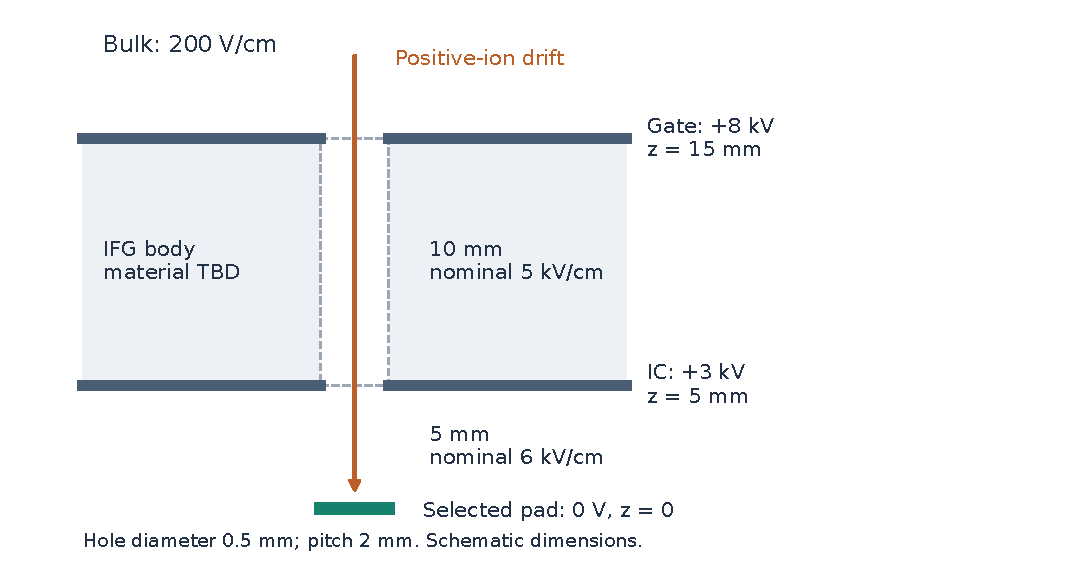
\includegraphics[width=.94\linewidth]{geometry.pdf}
\caption{Local coordinate and voltage convention. The hole walls and IFG body
are schematic; their material and electrical treatment remain unresolved.
The drawing does not represent a solved electric field.}
\label{fig:geometry}
\end{figure}

With the pad at zero, the IC is at $+3$ kV and the gate at $+8$ kV. The nominal
potential gradients are
\begin{equation}
 E_{\rm h}=\frac{8-3\ \mathrm{kV}}{10\ \mathrm{mm}}
 =5\ \mathrm{kV/cm},\qquad
 E_{\rm g}=\frac{3\ \mathrm{kV}}{5\ \mathrm{mm}}
 =6\ \mathrm{kV/cm}.
\end{equation}
These are field magnitudes; the axial physical electric field points downward.
Within and around real apertures the field is nonuniform. Dividing a voltage
drop by a distance supplies a nominal scale, not an aperture-field solution.

\clearpage
\subsection{Focusing must be checked at the entrance}
For circular holes of diameter $d_h$ on a square pitch $p$, the open fraction is
\begin{equation}
 f=\frac{\pi(d_h/2)^2}{p^2}=\OpenFraction.
\end{equation}
If all electric flux through one drift-region cell is to pass through its hole,
the simplified flux budget requires
\begin{equation}
 E_{\rm h} A_h\gtrsim E_{\rm d}p^2,
 \qquad E_{\rm h}\gtrsim\frac{E_{\rm d}}{f}
 =\EntranceThreshold\ \mathrm{kV/cm}.
 \label{eq:focus}
\end{equation}
Here the incident field is the \emph{bulk} field, $E_{\rm d}=200$ V/cm. Applying
this check at a different interface would miss the entrance bottleneck. The
nominal revised design gives $fE_{\rm h}/E_{\rm d}=\FluxRatio$, above unity.

Equation~\eqref{eq:focus} is a flux-capacity check under a simplified cell model.
It does not establish unit ion transparency. Field lines can terminate on grid
metal, diffusion can carry ions into walls, and material boundaries and alignment
can alter the collection map. The larger downstream nominal field supports
confinement of the exiting flux; it does not prove that every exiting ion lands
on the intended metal pad.

\section{Nominal transport and diffusion}
\subsection{Mobility inferred from the bulk operating point}
The working drift law is $v=\mu E$. The stated bulk speed implies
\begin{equation}
 \mu=\frac{0.1\ \mathrm{m/s}}{2.0\times10^4\ \mathrm{V/m}}
 =\Mobility\times10^{-6}\ \mathrm{m^2/(V\,s)}
 =0.05\ \mathrm{cm^2/(V\,s)}.
\end{equation}
This is the mobility at the working gas density; it is not the reduced mobility
normalized to a reference pressure. Extrapolating it unchanged to the IFG and
gap is an explicit approximation. The assumption must be checked against
mobility data over the relevant reduced-field range.

\begin{table}[ht]
\centering\small
\begin{tabular}{lrrrr}
\toprule
Region & $E$ (kV/cm) & $E/p$ (kV/cm/bar) & $v$ (m/s) & $t$ (ms) \\
\midrule
Bulk reference & 0.2 & 0.0133 & 0.1 & 15000.000 \\
IFG hole & 5 & 0.3333 & 2.5 & 4.000 \\
Collection gap & 6 & 0.4000 & 3 & 1.667 \\
\bottomrule
\end{tabular}

\caption{Uniform-field estimates using the same mobility in each region.
Reduced fields use the design pressure of 15 bar. The bulk reference path is
1.5 m, whereas the hole and gap paths are 10 and 5 mm respectively.}
\label{tab:regions}
\end{table}

The nominal IFG and gap transit times are therefore 4.0 and 1.67 ms. Their sum
is a common final-transport delay for otherwise identical trajectories. Neither
this sum nor the 15 s full bulk drift is the duration of a single-pad current
pulse. The pulse duration also depends on where the pad weighting potential
changes along the trajectory.

\clearpage
\subsection{Thermal diffusion as a reference model}
In the thermal, isotropic limit, the Einstein relation gives
\begin{equation}
 D=\frac{\mu k_BT}{e}=\DiffusionCoefficient\times10^{-7}\ \mathrm{m^2/s}.
\end{equation}
For a uniform drift distance $L$, the one-coordinate RMS spatial spread is
\begin{equation}
 \sigma=\sqrt{2Dt_d}
       =\sqrt{\frac{2k_BT}{e}\frac{L}{E}},\qquad t_d=\frac{L}{v}.
 \label{eq:diffusion}
\end{equation}
The thermal transverse form is also used in the ITACA design discussion
\cite{itaca2026}. Here $\sigma$ denotes one Cartesian coordinate, not the
two-dimensional radial RMS, which would be $\sqrt{2}\sigma$ for an isotropic
Gaussian. Taking the same coefficient longitudinally is an additional
thermal-isotropy assumption.

For one-dimensional constant drift and diffusion toward an absorbing plane,
the first-passage-time distribution has mean $L/v$ and variance $2DL/v^3$.
Equivalently, its RMS time spread is
\begin{equation}
 \sigma_t=\frac{\sigma_L}{v}.
 \label{eq:time_spread}
\end{equation}
The distribution is well approximated by a Gaussian when its relative width
is small. These formulas describe bulk transport; they are not a prescription
for transporting a covariance matrix through a nonuniform focusing field.

\begin{table}[ht]
\centering
\begin{tabular}{rrrr}
\toprule
$L$ (m) & $t_d$ (s) & $\sigma$ (mm) & $\sigma_t$ (ms) \\
\midrule
0.1 & 1 & 0.503 & 5.026 \\
0.75 & 7.5 & 1.376 & 13.765 \\
1.5 & 15 & 1.947 & 19.466 \\
\bottomrule
\end{tabular}

\caption{Thermal bulk-diffusion benchmark at 293.15 K and 200 V/cm. The arrival
time spread uses the bulk speed of 0.1 m/s.}
\end{table}

\begin{figure}[ht]
\centering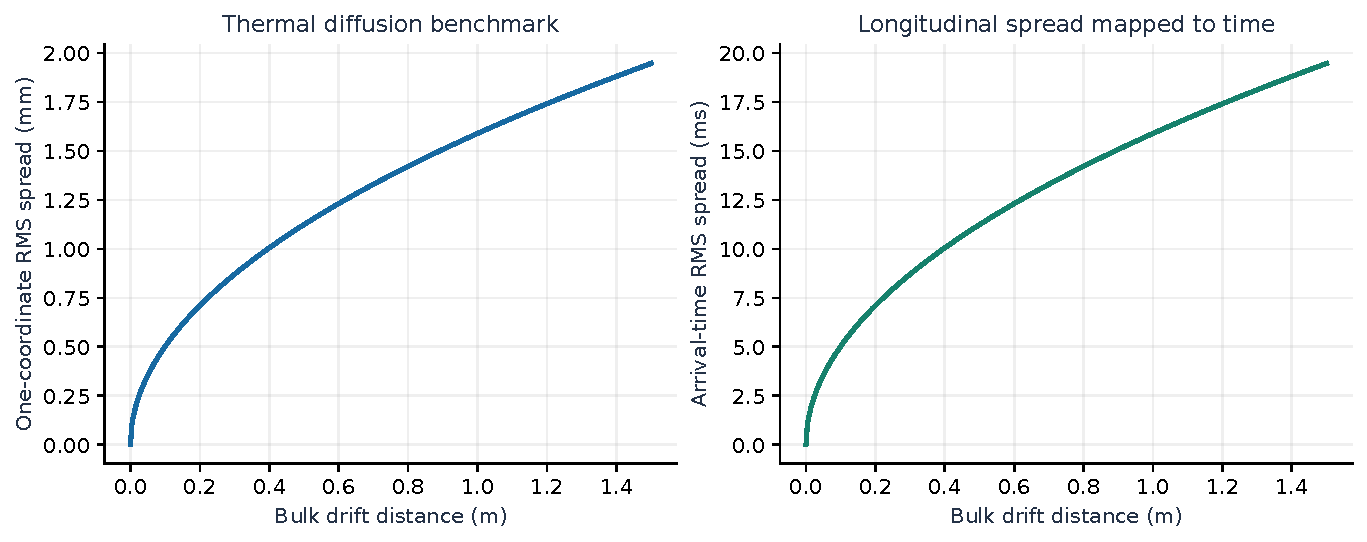
\includegraphics[width=\linewidth]{transport.pdf}
\caption{Spatial and temporal diffusion scales before the IFG. These are
calculated reference values, not measurements of ion transport.}
\end{figure}

A millimetre of longitudinal spread corresponds to 10 ms of arrival-time spread
at the bulk drift speed. Applying the faster gap velocity to that upstream
spread would incorrectly compress the arrival interval: ions entering the
same final trajectory at different times retain that time separation. The
focusing map and additional diffusion in the final regions require trajectory
transport to be treated quantitatively.

\clearpage
\section{Weighting potential and the single-ion signal}
\subsection{Two distinct electrostatic problems}
The physical potential $V$ determines ion trajectories through
$\mathbf E=-\nabla V$ and, in this approximation, $\mathbf v=\mu\mathbf E$.
It uses the actual electrode voltages. The weighting potential $\phi_w$ for one
readout pad instead satisfies
\begin{equation}
 \nabla\!\cdot\!\bigl(\epsilon(\mathbf r)\nabla\phi_w\bigr)=0,
 \qquad
 \phi_w=\begin{cases}1&\text{selected pad},\\0&\text{all other fixed-potential electrodes}.
 \end{cases}
 \label{eq:weighting}
\end{equation}
The ion is removed from this auxiliary problem. Dielectric interfaces obey
continuity of potential and of normal displacement in the absence of an imposed
free surface charge. Geometry, materials and boundary conditions determine
$\phi_w$; changing the applied biases alone does not change this weighting
potential. Floating or resistive electrodes would require a more general
treatment~\cite{riegler2016,riegler2019}.

With $\mathbf E_w=-\nabla\phi_w$ and our current convention,
\begin{align}
 i_p(t)&=q\frac{\dd\phi_w(\mathbf r(t))}{\dd t}
       =-q\,\mathbf v(t)\cdot\mathbf E_w(\mathbf r(t)),\label{eq:ramo}\\
 \int_{t_a}^{t_b}i_p(t)\,\dd t
       &=q\left[\phi_w(\mathbf r(t_b))-\phi_w(\mathbf r(t_a))\right].
       \label{eq:charge}
\end{align}
In this normalization $\phi_w$ is dimensionless and $\mathbf E_w$ has units
of inverse length. An ion starting where $\phi_w$ is negligible and reaching
the selected pad therefore gives an integrated signal of approximately $e$.
Neighboring pads can have transient induced currents even if they do not
collect the ion; their net signal is zero when both endpoint weighting
potentials are zero.

The ion induces current while approaching the electrode. After collection
its macroscopic drift contribution ceases. A separate extra charge-$e$ impulse
at impact would double count the charge already included in
Eq.~\eqref{eq:charge}. Microscopic surface processes are outside this model.

\subsection{What the focusing grid changes}
The fixed-potential grid screens the pad's weighting potential in the upstream
volume, with leakage through its apertures. The extent of that screening must
be calculated for the actual structure. This note does not assume an exact zero
weighting potential above a perforated grid. The current near a small pad is
generally not described by $qv/d$ with the full chamber drift length $d$.
That familiar expression follows from a uniform weighting field between broad
parallel electrodes, for which $\phi_w$ varies linearly across their separation.

The use of electrostatics is a quasistatic approximation. A light-propagation
time $d/c$ is not an ion-current rise time in this model; the waveform is set
by charge motion through the weighting field.

\clearpage
\section{Analytical central-pad benchmark}
\subsection{Boundary conditions and derivation}
Consider a square pad of side $2a$ in the plane $z=0$, set to unit weighting
potential. The remainder of that infinite plane is a grounded conductor. The
upper half-space is a homogeneous dielectric, with potential tending to zero
at infinity. This replaces the real IFG and dielectric stack by a tractable
reference boundary-value problem.

The half-space Poisson kernel gives~\cite{salazar2021}
\begin{equation}
 \phi_w(x,y,z)=\frac{1}{2\pi}\int_{-a}^{a}\!\int_{-a}^{a}
 \frac{z\,\dd x'\,\dd y'}{[(x-x')^2+(y-y')^2+z^2]^{3/2}}.
 \label{eq:poisson}
\end{equation}
It is the solid angle subtended by the pad divided by $2\pi$. Evaluating the
integral on the central axis yields
\begin{equation}
 \boxed{\phi_w(z)=\frac{2}{\pi}\tan^{-1}
 \left[\frac{a^2}{z\sqrt{z^2+2a^2}}\right]},\qquad z>0,
 \label{eq:square_phi}
\end{equation}
with the limiting value $\phi_w(0)=1$. Its positive normal weighting field is
\begin{equation}
 W(z)=-\frac{\dd\phi_w}{\dd z}
 =\frac{4a^2}{\pi(z^2+a^2)\sqrt{z^2+2a^2}}.
 \label{eq:square_field}
\end{equation}
The implemented formula is independently compared with numerical evaluation
of Eq.~\eqref{eq:poisson}. At large $z$, $\phi_w\simeq2a^2/(\pi z^2)$ and
$W\simeq4a^2/(\pi z^3)$; the pad response is concentrated near the metal.

For a central normal trajectory at constant speed $v$, let collection occur
at $t=0$. Then $z=-vt$ before collection and
\begin{equation}
 i_1(t)=\begin{cases} ev\,W(-vt),&t<0,\\0,&t\geq0.\end{cases}
 \label{eq:pulse}
\end{equation}
The one-sided value immediately before collection is
\begin{equation}
 i_1(0^-)=\frac{2\sqrt{2}}{\pi}\frac{ev}{a}.
\end{equation}
The step to zero idealizes collection at the metal and infinite readout
bandwidth. The smooth approach is a drift-averaged current; it does not resolve
individual gas collisions or atomic-scale image-force dynamics.

The pulse scales as $i_{\rm peak}\propto v/a$ and duration $\propto a/v$, while
its full integrated charge is $e$. The same constant-speed benchmark extended
to $t=-\infty$ has a mathematically integrable tail. That extension must not be
interpreted as the real trajectory through the upstream grid.

\clearpage
\subsection{Numbers, duration definitions and finite-path charge}
Using $a=\SquareHalfWidth$ mm and $v=\GapSpeed$ m/s gives the results in
Table~\ref{tab:pulse}. To define charge-based durations, invert the potential:
\begin{equation}
 z(\phi)=a\sqrt{\frac{1}{\sin(\pi\phi/2)}-1}.
\end{equation}
The cumulative full-path signal fraction before collection is $\phi_w(z)$.
The final interval containing fraction $F$ of the signal has duration
$z(1-F)/v$. The central 90\% interval instead runs from cumulative fractions
0.05 to 0.95. These durations differ from the time above half peak; none is an
exponential decay constant.

\begin{table}[ht]
\centering\small
\begin{tabular}{lr}
\toprule
Quantity & Value \\
\midrule
Peak immediately before collection & 1.731 fA \\
Characteristic time $a/v$ & 83.33 $\mu$s \\
Time above half peak & 70.52 $\mu$s \\
Final interval containing 90\% of charge & 193.51 $\mu$s \\
Final interval containing 99\% of charge & 659.67 $\mu$s \\
Central 90\% interval (5--95\%) & 280.96 $\mu$s \\
Cumulative charge 10--90\% rise & 184.21 $\mu$s \\
Charge induced from 5 mm to the metal & 0.9984124 $e$ \\
\bottomrule
\end{tabular}

\caption{Central square-pad benchmark. Full-path fractional durations refer to
the ideal half-space model, without electronic shaping.}
\label{tab:pulse}
\end{table}

\begin{figure}[ht]
\centering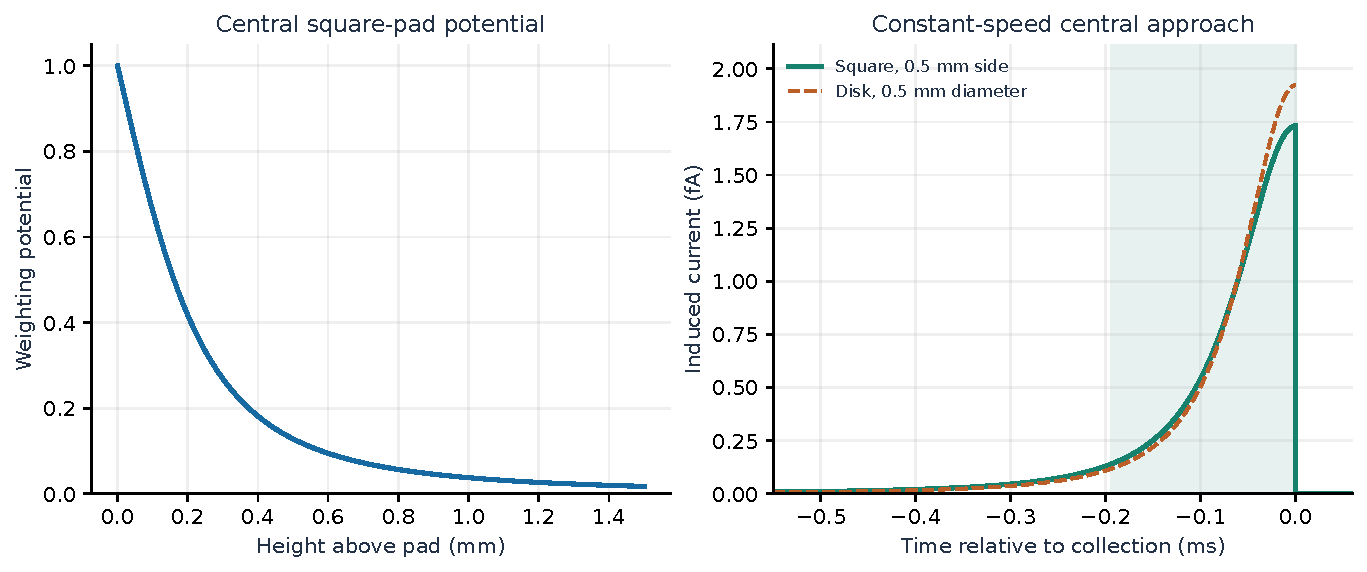
\includegraphics[width=\linewidth]{single_ion.pdf}
\caption{Analytical weighting potential and current. The shaded interval
contains the final 90\% of the square-pad signal. The circular-pad comparison
uses the same grounded-plane assumption and the same lateral diameter as the
square side. The physical geometry is not resolved by either model.}
\end{figure}

For a trajectory beginning at the nominal gap height $g=5$ mm,
\begin{equation}
 \phi_w(g)=\GapPotential,\qquad
 Q_{g\to0}=e[1-\phi_w(g)]=\GapChargeFraction\,e.
\end{equation}
The missing \GapMissingPercent\% belongs to the earlier part of this idealized
trajectory. It is not discarded or reassigned by normalization. A full IFG
solution will distribute the entire signal according to its own weighting
potential and trajectory. Small $\phi_w(g)$ in this model does not bound the
error from different pad surroundings or dielectric boundaries.

\clearpage
\subsection{Geometry dependence and an independent shape comparison}
For a circular pad of radius $a$ in the same infinite grounded plane, direct
integration of the Poisson kernel gives
\begin{equation}
 \phi_{w,\circ}(z)=1-\frac{z}{\sqrt{z^2+a^2}},\qquad
 W_\circ(z)=\frac{a^2}{(z^2+a^2)^{3/2}}.
\end{equation}
Its central peak is $ev/a=\DiskPeakCurrent$ fA for diameter 0.5 mm, compared
with \PeakCurrent\ fA for the 0.5 mm square. This difference is a comparison
of two specified boundary problems, not a systematic uncertainty estimate for
the actual pad. Off-centre trajectories and ideal sharp edges can change the
local peak appreciably; finite electrode edges, gaps and dielectrics matter.

\begin{table}[ht]
\centering
\begin{tabular}{rrr}
\toprule
$z$ (mm) & $\phi_w(z)$ & $i(z)$ (fA) \\
\midrule
5 & 0.001588 & 0.000304 \\
1 & 0.037470 & 0.033940 \\
0.5 & 0.128188 & 0.199874 \\
0.25 & 0.333333 & 0.706661 \\
0.1 & 0.661663 & 1.435876 \\
0.05 & 0.822863 & 1.647985 \\
0 & 1.000000 & 1.730959 \\
\bottomrule
\end{tabular}

\caption{Square-pad sensitivity and central current at selected heights. The
row at $z=0$ gives the pre-collection limit, not the current after absorption.}
\end{table}

An unknown region between pads cannot be assigned a zero weighting potential
merely because neighboring pads are at zero in the auxiliary problem. A
grounded metal plane enforces a Dirichlet boundary; an exposed dielectric
requires a dielectric-interface solution. This distinction is likely more
important than the square-versus-disk comparison. The present benchmark has
no quantitative uncertainty envelope for that missing geometry.

\section{Implications for the next physics milestone}
The ion trajectory takes milliseconds through the last structures, while the
central benchmark induces most of its pad signal in a fraction of a millisecond.
Bulk diffusion can spread arrivals over tens of milliseconds. These are three
different timescales. A many-ion input is the sum of the appropriate single-ion
signals, each placed at its own collection time.

For a curved event, depth orders arrival time. Total electron path length does
not fix the time span on one pad. The 10 cm straight segment aligned with drift
is retained only as a diagnostic extreme. Realistic calculations must preserve
the event's isotropic orientation, scattering, nonuniform deposition, endpoint
blobs and repeated intersections with a pad's collection region.

\clearpage
\section{Validation, reproduction and remaining work}
The automated suite contains independent physical checks:
\begin{enumerate}
\item The nominal voltage drops and region lengths reproduce the revised fields.
\item The thermal spread agrees with both $\sqrt{2Dt}$ and the uniform-drift
first-passage time variance.
\item Numerical surface integration reproduces the square-pad potential.
\item A finite-difference derivative reproduces the analytical weighting field;
surface and far-field limits and monotonicity are checked.
\item Independent quadrature gives unit full-path weighting-field integral,
and the finite-gap integral equals its endpoint potential difference.
\item Velocity scaling preserves charge and stretches time inversely; sampled
spatial integration converges as its step is reduced.
\end{enumerate}
Passing these checks establishes implementation consistency. It does not
measure ion transparency, real drift coefficients, or the actual ASIC response.

From the repository root, the reproducible entry points are
\begin{verbatim}
make PYTHON=<python-with-dependencies> test physics
make PYTHON=<python-with-dependencies> note
\end{verbatim}
The scripts read \texttt{config/detector.toml}; numerical results and environment
versions are saved in \texttt{results/physics\_benchmarks.json}. This note
includes generated figures, tables and value macros. The configuration hash
prefix for the present build is \texttt{\ConfigHash}. The analytical model is
deterministic and has no random seed.

Before replacing the benchmarks with a detector prediction, establish the pad
outline, surrounding metallization and guard electrodes; the IFG wall material
and metallization; the dielectric stack; and alignment and edge geometry.
Obtain or justify mobility and longitudinal/transverse diffusion over the
operating reduced fields. Solve the physical and weighting fields separately,
checking domain and mesh convergence and integral charge identities.

The next stage will map three-dimensional energy deposits into pad-specific
arrival distributions, then into current waveforms. Packet charge, central-90\%
duration, peak current, repeated-packet separation and charge per readout bin
will form the interface to the electronics study. Feedback-retention
requirements and the properties of Rogelio's feedback transistor remain outside
the present milestone.

\bibliographystyle{unsrtnat}
\bibliography{references}
\end{document}
